% !TEX TS-program = knitr
\documentclass[handout]{beamer}\usepackage{graphicx, color}
%% maxwidth is the original width if it is less than linewidth
%% otherwise use linewidth (to make sure the graphics do not exceed the margin)
\makeatletter
\def\maxwidth{ %
  \ifdim\Gin@nat@width>\linewidth
    \linewidth
  \else
    \Gin@nat@width
  \fi
}
\makeatother

\IfFileExists{upquote.sty}{\usepackage{upquote}}{}
\definecolor{fgcolor}{rgb}{0.2, 0.2, 0.2}
\newcommand{\hlnumber}[1]{\textcolor[rgb]{0,0,0}{#1}}%
\newcommand{\hlfunctioncall}[1]{\textcolor[rgb]{0.501960784313725,0,0.329411764705882}{\textbf{#1}}}%
\newcommand{\hlstring}[1]{\textcolor[rgb]{0.6,0.6,1}{#1}}%
\newcommand{\hlkeyword}[1]{\textcolor[rgb]{0,0,0}{\textbf{#1}}}%
\newcommand{\hlargument}[1]{\textcolor[rgb]{0.690196078431373,0.250980392156863,0.0196078431372549}{#1}}%
\newcommand{\hlcomment}[1]{\textcolor[rgb]{0.180392156862745,0.6,0.341176470588235}{#1}}%
\newcommand{\hlroxygencomment}[1]{\textcolor[rgb]{0.43921568627451,0.47843137254902,0.701960784313725}{#1}}%
\newcommand{\hlformalargs}[1]{\textcolor[rgb]{0.690196078431373,0.250980392156863,0.0196078431372549}{#1}}%
\newcommand{\hleqformalargs}[1]{\textcolor[rgb]{0.690196078431373,0.250980392156863,0.0196078431372549}{#1}}%
\newcommand{\hlassignement}[1]{\textcolor[rgb]{0,0,0}{\textbf{#1}}}%
\newcommand{\hlpackage}[1]{\textcolor[rgb]{0.588235294117647,0.709803921568627,0.145098039215686}{#1}}%
\newcommand{\hlslot}[1]{\textit{#1}}%
\newcommand{\hlsymbol}[1]{\textcolor[rgb]{0,0,0}{#1}}%
\newcommand{\hlprompt}[1]{\textcolor[rgb]{0.2,0.2,0.2}{#1}}%

\usepackage{framed}
\makeatletter
\newenvironment{kframe}{%
 \def\at@end@of@kframe{}%
 \ifinner\ifhmode%
  \def\at@end@of@kframe{\end{minipage}}%
  \begin{minipage}{\columnwidth}%
 \fi\fi%
 \def\FrameCommand##1{\hskip\@totalleftmargin \hskip-\fboxsep
 \colorbox{shadecolor}{##1}\hskip-\fboxsep
     % There is no \\@totalrightmargin, so:
     \hskip-\linewidth \hskip-\@totalleftmargin \hskip\columnwidth}%
 \MakeFramed {\advance\hsize-\width
   \@totalleftmargin\z@ \linewidth\hsize
   \@setminipage}}%
 {\par\unskip\endMakeFramed%
 \at@end@of@kframe}
\makeatother

\definecolor{shadecolor}{rgb}{.97, .97, .97}
\definecolor{messagecolor}{rgb}{0, 0, 0}
\definecolor{warningcolor}{rgb}{1, 0, 1}
\definecolor{errorcolor}{rgb}{1, 0, 0}
\newenvironment{knitrout}{}{} % an empty environment to be redefined in TeX

\usepackage{alltt}
\newcommand{\answers}{1}

\setbeamercovered{dynamic}
\usetheme{Marburg}
\setbeamertemplate{navigation symbols}{} 
\setbeamertemplate{footline}
{
  \leavevmode%
  \hbox{%
  \begin{beamercolorbox}[wd=.333333\paperwidth,ht=2.25ex,dp=1ex,center]{author in head/foot}%
    \usebeamerfont{author in head/foot}\copyright $\ $ \insertshortauthor%~~\beamer@ifempty{\insertshortinstitute}{}{(\insertshortinstitute)}
  \end{beamercolorbox}%
  \begin{beamercolorbox}[wd=.333333\paperwidth,ht=2.25ex,dp=1ex,center]{title in head/foot}%
    \usebeamerfont{title in head/foot} \insertinstitute
  \end{beamercolorbox}%
  \begin{beamercolorbox}[wd=.333333\paperwidth,ht=2.25ex,dp=1ex,right]{date in head/foot}%
    \usebeamerfont{date in head/foot}\insertshortdate{}\hspace*{2em}
    \insertframenumber{} / \inserttotalframenumber\hspace*{2ex} 
  \end{beamercolorbox}}%
  \vskip0pt%
}

\usepackage{amsmath}
\usepackage{caption}
\usepackage{color}
\usepackage{enumerate}
\usepackage{listings}
\usepackage{hyperref}
\usepackage{mathrsfs}
\usepackage{natbib}
\usepackage{url}

\providecommand{\all}{\ \forall \ }
\providecommand{\bs}{\backslash}
\providecommand{\e}{\varepsilon}
\providecommand{\E}{\ \exists \ }
\providecommand{\lm}[2]{\lim_{#1 \rightarrow #2}}
\providecommand{\m}[1]{\mathbb{#1}}
\providecommand{\nv}{{}^{-1}}
\providecommand{\ov}[1]{\overline{#1}}
\providecommand{\p}{\newpage}
\providecommand{\q}{$\quad$ \newline}
\providecommand{\rt}{\rightarrow}
\providecommand{\Rt}{\Rightarrow}
\providecommand{\vc}[1]{\boldsymbol{#1}}
\providecommand{\wh}[1]{\widehat{#1}}

\hypersetup{colorlinks,linkcolor=,urlcolor=blue}
\numberwithin{equation}{section}

\definecolor{dkgreen}{rgb}{0,0.6,0}
\definecolor{gray}{rgb}{0.5,0.5,0.5}
\definecolor{mauve}{rgb}{0.58,0,0.82}

\lstset{ 
  language=C,                % the language of the code
  basicstyle= \footnotesize,           % the size of the fonts that are used for the code
  numberstyle= \tiny \color{white},  % the style that is used for the line-numbers
  stepnumber=2,                   % the step between two line-numbers. 
  numbersep=5pt,                  % how far the line-numbers are from the code
  backgroundcolor=\color{white},      % choose the background color. You must add \usepackage{color}
  showspaces=false,               % show spaces adding particular underscores
  showstringspaces=false,         % underline spaces within strings
  showtabs=false,                 % show tabs within strings adding particular underscores
  frame=lrb,                   % adds a frame around the code
  rulecolor=\color{black},        % if not set, the frame-color may be changed on line-breaks within not-black text 
  tabsize=2,                      % sets default tabsize to 2 spaces
  captionpos=t,                   % sets the caption-position 
  breaklines=true,                % sets automatic line breaking
  breakatwhitespace=false,        % sets if automatic breaks should only happen at whitespace
  %title=\lstname,                   % show the filename of files included with \lstinputlisting;
  keywordstyle=\color{blue},          % keyword style
  commentstyle=\color{gray},       % comment style
  stringstyle=\color{dkgreen},         % string literal style
  escapeinside={\%*}{*)},            % if you want to add LaTeX within your code
  morekeywords={*, ...},               % if you want to add more keywords to the set
  xleftmargin=0.053in, % left horizontal offset of caption box
  xrightmargin=-.03in % right horizontal offset of caption box
}

%\DeclareCaptionFont{white}{\color{white}}
%\DeclareCaptionFormat{listing}{\parbox{\textwidth}{\colorbox{gray}{\parbox{\textwidth}{#1#2#3}}\vskip-0.05in}}
%\captionsetup[lstlisting]{format = listing, labelfont = white, textfont = white}
%For caption-free listings, comment out the 3 lines above and uncomment the 2 lines below.
 \captionsetup{labelformat = empty, labelsep = none}
 \lstset{frame = single}




\title{More on Confidence Intervals}
\author{Will Landau}
\date{Mar 28, 2013}
\institute{Iowa State University}

\begin{document}

\begin{frame}
\titlepage
 \end{frame}
 
 \AtBeginSection[]
{
   \begin{frame}
       \frametitle{Outline}
       \tableofcontents[currentsection]
   \end{frame}
}

\section{$n \ge 25$, $\sigma$ unknown}


\begin{frame}
\frametitle{$n \ge 25$, $\sigma$ unknown} \small
\begin{itemize}
\item The formula for a 2-sided, $1 - \alpha$ CI for a true mean $\mu$ from before was:
\pause \begin{align*}
(\ov{x} - z_{1 - \alpha/2} \frac{\sigma}{\sqrt{n}}, \ \ov{x} + z_{1 - \alpha/2} \frac{\sigma}{\sqrt{n}})
\end{align*}
\pause \item If $n \ge 25$ and $\sigma$ is unknown, you can replace $\sigma$ in the confidence interval formula with the sample standard deviation, $s = \sqrt{\frac{1}{n-1} \sum_{i = 1}^n (x_i - \ov{x})^2}$.
\pause \item The formula for the 2-sided confidence interval becomes:
\pause \begin{align*}
(\ov{x} - z_{1 - \alpha/2} \frac{s}{\sqrt{n}}, \ \ov{x} + z_{1 - \alpha/2} \frac{s}{\sqrt{n}})
\end{align*}
\pause \item The analogous upper and lower confidence intervals, respectively, are:
\begin{align*}
&\uncover<7->{(-\infty, \ \ov{x} + z_{1 - \alpha} \frac{s}{\sqrt{n}})} \\
&\uncover<8->{(\ov{x} - z_{1 - \alpha} \frac{s}{\sqrt{n}}, \ \infty)}
\end{align*}
\end{itemize}
\end{frame}

\begin{frame}
\frametitle{Your turn: breaking strength of wire}
\begin{itemize}
\item Suppose you are a manufacturer of construction equipment. You make 0.0125 inch wire rope and need to determine how much weight it can hold before breaking so that you can label it clearly.
\pause \item Here are breaking strengths, in kg, for 40 sample wires:
\end{itemize}
\setkeys{Gin}{width=1\textwidth} 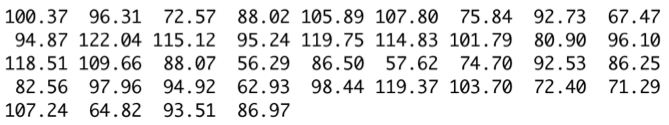
\includegraphics{../../fig/wiredata.png}
\begin{itemize}
\pause \item The sample mean breaking strength is $91.85$ kg and the sample standard deviation is 17.79 kg. 
\pause \item Using the appropriate 95\% confidence interval, try to determine whether the breaking strengths is meet the requirement of 85 kg.
\end{itemize}
\end{frame}

\begin{frame}<handout:\answers>
\frametitle{Answers: breaking strength of wire} \small
\begin{itemize}
\item Since we want the breaking strengths to be above 85 kg, I choose a lower confidence interval (one with a lower bound).
\pause \item $\alpha = 1 -0.95 = 0.05$, $\ov{x} = 91.85$, $s = 17.79$, and $n = 40$.
\begin{align*}
\uncover<3->{(\ov{x} -}&\uncover<3->{ z_{1 - \alpha} \frac{s}{\sqrt{n}}, \ \infty)} \\
&\uncover<4->{= \left (91.85 - z_{1 - 0.05} \frac{17.79}{\sqrt{40}}, \ \infty \right)} \\
&\uncover<5->{= (91.85 - z_{0.95} \cdot 2.81, \ \infty)} \\
&\uncover<6->{= (91.85 - 1.64 \cdot 2.81, \ \infty)} \\
&\uncover<7->{= (87.24, \ \infty)}
\end{align*}
\uncover<8->{\item With 95\% confidence, we have shown that the true mean breaking strength is above 87.24 kg. Hence, we meet the 85 kg requirement with 95\% confidence.}
\uncover<9->{\item What is the maximum confidence level with which we can meet the 85kg requirement?}
\end{itemize}
\end{frame}


\begin{frame}<handout:\answers>
\frametitle{Answers: breaking strength of wire} \scriptsize
\begin{itemize}
\item The confidence interval is:
\pause \begin{align*}
(91.85 - z_{1 - \alpha} \cdot 2.81, \ \infty)
\end{align*}
\pause \item To meet the requirement, we need 
\begin{align*}
\uncover<4->{91.85 - z_{1 - \alpha} \cdot 2.81} & \uncover<4->{< 85} \\
\uncover<5->{z_{1-\alpha}} & \uncover<5->{< \frac{6.85}{ 2.81}} \\
&\uncover<6->{= 2.44} \\
\uncover<7->{\Phi(z_{1 - \alpha})} & \uncover<7->{< \Phi(2.44)} \\
\uncover<8->{1 - \alpha} & \uncover<8->{< 0.9926}
\end{align*}
\uncover<9->{\item Hence, we could have raised the confidence level up to 99.26 \% and still shown that we met the requirement.}
\uncover<10->{\item (In hypothesis testing, which will come later, $1 - 0.9926 = 0.0074$ will be a {\bf p-value}.)}
\uncover<11->{\item Now, calculate and interpret a 95\%, 2-sided confidence interval for the true mean breaking strength. Is there any reason to \emph{disbelieve} that the true mean breaking strength is 94 kg?}
\end{itemize}
\end{frame}

\begin{frame}<handout:\answers>
\frametitle{Answers: breaking strength of wire}
\begin{itemize}
\item The two-sided confidence interval is:
\begin{align*}
\uncover<2->{(\ov{x}} & \uncover<2->{-z_{1 - \alpha/2} \frac{s}{\sqrt{n}}, \ \ov{x} + z_{1 - \alpha/2} \frac{s}{\sqrt{n}})} \\
&\uncover<3->{=\left (91.85 - z_{1 - 0.05/2} \frac{17.79}{\sqrt{40}}, \ 91.85 + z_{1 - 0.05/2} \frac{17.79}{\sqrt{40}} \right )} \\
&\uncover<4->{=(91.85 - z_{0.975} \cdot 2.81, \ 91.85 + z_{0.975} \cdot 2.81)} \\
&\uncover<5->{=(91.85 - 1.96\cdot 2.81, \ 91.85  + 1.96 \cdot 2.81)} \\
&\uncover<6->{=(86.34, 97.36)}
\end{align*}
\uncover<7->{\item With 95\% confidence, the true mean breaking strength is between 86.34 kg and 97.36 kg.}
\uncover<8->{\item Since 94 kg is in the interval, at $\alpha = 0.05$, we have no evidence to dispute the claim that the true mean breaking strength is 94 kg.}
\end{itemize}
\end{frame}


\section{$n < 25$, $\sigma$ unknown}

\begin{frame}
\frametitle{$n < 25, \ \sigma$ unknown}
\begin{itemize}
\item We need to assume that $X_1, \ldots, X_n$ are not only iid with mean $\mu$ and variance $\sigma^2$, but also that these random variables are \emph{normally distributed}.
\begin{itemize}
\pause \item We can't use the Central Limit Theorem since $n < 25$. 
\pause \item However, the additional assumption makes $\ov{X}$ normally distributed (A linear combination of \emph{independent} normal random variables is normal.)
\end{itemize}
\pause \item We need to use the $t_{n - 1, 1 - \alpha/2}$ instead of $z_{1 - \alpha/2}$ in the confidence intervals
\begin{itemize}
\pause \item Although $\frac{\ov{X} - \mu}{\sigma/\sqrt{n}} \sim N(0,1)$, it's a fact that $\frac{\ov{X} - \mu}{s/\sqrt{n}} \sim t_{n - 1}$ since $s$ is random ($(n-1)s^2/\sigma^2 \sim \chi^2_{n-1}$).
\pause \item For $n < 25$, the $t_{n - 1}$ distribution is \emph{not} close enough to N(0,1).
\end{itemize}
\end{itemize}
\end{frame}


\begin{frame}
\frametitle{New confidence interval formulas for $n < 25, \ \sigma$ unknown}
\begin{itemize}
\item Two-sided $1 - \alpha$ CI:
\pause \begin{align*}
(\ov{x} - t_{n - 1, \ 1 - \alpha/2} \frac{s}{\sqrt{n}},\ \ov{x} + t_{n - 1, \ 1- \alpha/2 } \frac{s}{\sqrt{n}})
\end{align*} 
\pause \item One-sided lower $1 - \alpha$ CI:
\pause \begin{align*}
(\ov{x} - t_{n - 1, \ 1 - \alpha} \frac{s}{\sqrt{n}}, \ \infty)
\end{align*} 
\pause \item One-sided upper $1 - \alpha$ CI:
\pause \begin{align*}
(-\infty, \ \ov{x} + t_{n - 1, \ 1- \alpha } \frac{s}{\sqrt{n}})
\end{align*} 
\end{itemize}
\end{frame}


\begin{frame}
\frametitle{Your turn: concrete beams}
\begin{itemize}
\item 10 concrete beams were each measured for flexural strength (MPa):
\begin{center}
\setkeys{Gin}{width=.7\textwidth} 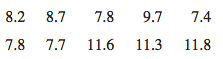
\includegraphics{../../fig/fbeams.png}
\end{center}
\pause \item Assuming the flexural strengths are iid normal, calculate and interpret a two-sided 99\% CI for the flexural strength of the beams.
\pause \item Is the true mean flexural strength below the minimum requirement of 11 MPa? Find out with the appropriate 95\% CI.
\end{itemize}
\end{frame}

\begin{frame}<handout:\answers>
\frametitle{Answers: concrete beams} \scriptsize
\begin{itemize}
\item $n = 10$, $\alpha = 0.01$
\pause \item $\ov{x} = \frac{1}{10}(8.2 + 8.7 + \cdots + 11.8) = 9.2$
\pause \item $s = \sqrt{\frac{1}{10-1} [(8.7 - 9.2)^2 + (8.7 - 9.2)^2 + \cdots + (11.8-9.2)^2]} = 1.76$
\pause \item The two-sided 99\% CI is:
\begin{align*}
\uncover<5->{(\ov{x}}& \uncover<5->{ - t_{n - 1, \ 1 - \alpha/2} \frac{s}{\sqrt{n}},\ \ov{x} + t_{n - 1, \ 1- \alpha/2 } \frac{s}{\sqrt{n}})} \\
&\uncover<6->{= \left (9.2 - t_{10 - 1, \ 1 - 0.01/2} \frac{1.76}{\sqrt{10}}, \ 9.2 + t_{10 - 1, \ 1 - 0.01/2} \frac{1.76}{\sqrt{10}} \right )} \\
&\uncover<7->{= (9.2 - t_{9, 0.995} \cdot 0.556, \ 9.2 + t_{9, 0.995} \cdot 0.556)} \\
&\uncover<8->{= (9.2 - 3.250 \cdot 0.556, \ 9.2 + 3.250 \cdot 0.556)} \\
&\uncover<9->{= (7.393, \ 11.007)}
\end{align*}
\uncover<10->{\item We're 99\% confident that the true flexural strength of this kind of concrete beam is between 7.393 MPa and 11.007 MPa.}
\end{itemize}
\end{frame}

\begin{frame}<handout:\answers>
\frametitle{Answers: concrete beams}
\begin{itemize}
\item I want to know whether the true mean flexural strength is \emph{below} 11 MPa. Hence, I need an \emph{upper} 95\% confidence interval (i.e., with an upper bound). 
\begin{align*}
\uncover<2->{(-\infty,} &\uncover<2->{\ \ov{x} + t_{n - 1, \ 1- \alpha } \frac{s}{\sqrt{n}})} \\
&\uncover<3->{= (-\infty, \ 9.2 + t_{9, \ 1- 0.05 } \frac{1.76}{\sqrt{10}})} \\
&\uncover<4->{= (-\infty, \ 9.2 + t_{9, 0.95} \cdot 0.556)} \\
&\uncover<5->{= (-\infty, \ 9.2 + 1.83 \cdot 0.556)} \\
&\uncover<6->{= (-\infty, \ 10.21)}
\end{align*}
\uncover<7->{\item We're 95\% confident that the true mean flexural strength is below 10.21 MPa.} \uncover<8->{ That's below 11 MPa. So at $\alpha = 0.05$, we have shown that the true mean flexural strength is also below 11 MPa and the requirement is not met.}
\end{itemize}
\end{frame}


\begin{frame}
\frametitle{Your turn: paint thickness} \scriptsize
\begin{itemize}
\item Consider the following sample of observations on coating thickness for low-viscosity paint: \q
\begin{tabular}{cccccccc}
0.83 & 0.88 & 0.88 & 1.04 & 1.09 & 1.12 & 1.29 & 1.31 \\
1.48 & 1.49 & 1.59 & 1.62 & 1.65 & 1.71 & 1.76 & 1.83
\end{tabular} \q
\item A normal QQ plot shows that they are close enough to normally distributed. \q 
\begin{center}
\begin{knitrout}
\definecolor{shadecolor}{rgb}{0.969, 0.969, 0.969}\color{fgcolor}
\includegraphics[width=.4\textwidth,height=.4\textheight]{figure/unnamed-chunk-2} 

\end{knitrout}

\end{center}
\item Calculate and interpret a two-sided 90\% confidence interval for the true mean thickness.
\end{itemize}
\end{frame}

\begin{frame}<handout:\answers>
\frametitle{Answers: paint thickness} \scriptsize
\begin{itemize}
\item $n = 16$, $\alpha = 0.1$
\pause \item $\ov{x} = \frac{1}{16}(0.83 + 0.88 + \cdots + 1.83) = 1.35$ mm
\pause \item $s = \sqrt{\frac{1}{16-1} [(0.83 - 1.35)^2 + (0.88 - 1.35)^2 + \cdots + (1.83-1.35)^2]} = 0.34$ mm
\pause \item The two-sided 90\% CI is:
\begin{align*}
\uncover<5->{(\ov{x}}&\uncover<5->{ - t_{n - 1, \ 1 - \alpha/2} \frac{s}{\sqrt{n}},\ \ov{x} + t_{n - 1, \ 1- \alpha/2 } \frac{s}{\sqrt{n}})} \\
&\uncover<6->{= \left (1.35 - t_{10 - 1, \ 1 - 0.1/2} \frac{0.34}{\sqrt{16}}, \ 1.35 + t_{16 - 1, \ 1 - 0.1/2} \frac{0.34}{\sqrt{16}} \right )} \\
&\uncover<7->{= (1.35 - t_{15, 0.95} \cdot 0.085, \ 1.35 + t_{15, 0.95} \cdot0.085)} \\
&\uncover<8->{= (1.35 - 1.75 \cdot 0.085, \ 1.35 + 1.75 \cdot 0.085)} \\
&\uncover<9->{= (1.201, \ 1.499)}
\end{align*}
\uncover<10->{\item We're 90\% confident that the true mean thickness is between 1.201 mm and 1.499 mm.}
\end{itemize}

\end{frame}




\section{Hypothesis Testing with Confidence Intervals}
\begin{frame}
\frametitle{Statistical inference}
\begin{itemize}
\item {\bf Statistical inference}: using data from the sample to draw conclusions about the population 
\begin{itemize}
\pause \item Point estimation (confidence intervals): estimating population parameters and specifying the degree of precision of the estimate.
\pause \item Hypothesis testing: testing the validity of statements about the population that are framed in terms of parameters. 
\end{itemize}
\end{itemize}
\end{frame}

\begin{frame}
\frametitle{Hypothesis testing} \scriptsize
\begin{itemize}
\item {\bf Hypothesis testing (significance testing)}: the use of data in the quantitative assessment of the plausibility of some trial value or a parameter. 
\pause \item You have competing {\bf hypotheses}, or statements, about a population:
\begin{itemize}
\pause \item The {\bf null hypothesis}, denoted $H_0$ is the proposition that a parameter equals some fixed number.
\pause \item The {\bf alternative hypothesis}, denoted $H_a$ or $H_1$, is a statement that stands in opposition to the null hypothesis.
\pause \item Examples:\q
\setkeys{Gin}{width=.6\textwidth} 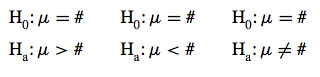
\includegraphics{../../fig/examplehypotheses.png}
\end{itemize}
\pause \item Note: $H_a: \mu \ne \#$ makes a {\bf two-sided test}, while $H_a: \mu < \#$ and $H_a: \mu > \#$ make a {\bf one-sided test}.
\pause \item The goal is to use the data to debunk the null hypothesis in favor of the alternative:
\begin{itemize}
\pause \item Assume $H_0$.
\pause \item Try to show that, under $H_0$, the data are preposterous.
\pause \item If the data are preposterous, reject $H_0$ and conclude $H_a$. Otherwise, fail to reject $H_0$.
\end{itemize}
\end{itemize}
\end{frame}

\begin{frame}
\frametitle{Hypothesis testing}
\begin{itemize}
\item Outcomes of a hypothesis test: \q
\setkeys{Gin}{width=.5\textwidth} 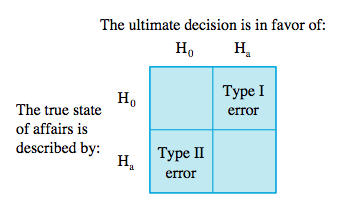
\includegraphics{../../fig/typeerrors.png}
\pause \item $\alpha$ (the very same $\alpha$ in confidence intervals) is the probability of rejecting $H_0$ when $H_0$ is true.
\begin{itemize}
\pause \item $\alpha$ is the Type I Error probability.
\pause \item For honesty's sake, $\alpha$ is fixed before you even \emph{look} at the data.
\end{itemize} 
\end{itemize}
\end{frame}

\begin{frame}
\frametitle{3 Methods of Hypothesis Testing}
\begin{enumerate}[1. ]
\item Confidence intervals
\pause \item Critical values
\pause \item P-values
\end{enumerate}
\end{frame}

\begin{frame}
\frametitle{Formal steps of a hypothesis test using confidence intervals}
\begin{enumerate}[1. ]
\item State the hypotheses, $H_0$ and $H_a$.
\pause \item State the significance level, $\alpha$.
\pause \item State the form of the $1 - \alpha$ confidence interval you will use, along with all the assumptions necessary. 
\begin{itemize}
\item The confidence interval should contain $\mu$ when there is little to no evidence against $H_0$ and should \emph{not} contain $\mu$ when there is strong evidence against $H_0$. 
\item Use one-sided confidence intervals for one-sided tests (i.e., $H_a: \mu < \#$ or $\mu > \#$) and two-sided intervals for two-sided tests ($H_a: \mu \ne \#$).
\end{itemize}
\pause \item Calculate the $1 - \alpha$ confidence interval.
\pause \item Based on the $1 - \alpha$ confidence interval, either:
\begin{itemize}
\pause \item Reject $H_0$ and conclude $H_a$, or
\pause \item Fail to reject $H_0$.
\end{itemize}
\pause \item Interpret the conclusion using layman's terms.
\end{enumerate}
\end{frame}


\begin{frame}
\frametitle{Example: breaking strength of wire}
\begin{itemize}
\item Suppose you are a manufacturer of construction equipment. You make 0.0125 inch wire rope and need to determine how much weight it can hold before breaking so that you can label it clearly.
\pause \item Here are breaking strengths, in kg, for 40 sample wires:
\end{itemize}
\setkeys{Gin}{width=1\textwidth} 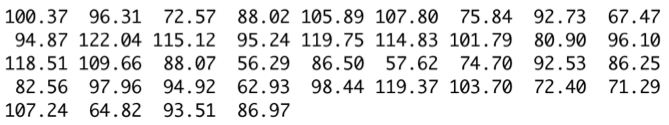
\includegraphics{../../fig/wiredata.png}
\begin{itemize}
\pause \item Let's conduct a hypothesis test to find out if the true mean breaking strength is above 85 kg.
\end{itemize}
\end{frame}

\begin{frame}
\frametitle{Example: breaking strength of wire} \scriptsize
\begin{enumerate}[1. ]
\item $H_0: \mu = 85$ kg and $H_a: \mu > 85$ kg, where $\mu$ is the true mean breaking strength.
\pause \item $\alpha$ = 0.05
\pause \item Since this is a one-sided (lower) test, I will use a lower $1 - \alpha$ confidence interval:
\pause \begin{align*}
\left (\ov{x} - z_{1 - \alpha} \frac{s}{\sqrt{n}}, \ \infty \right )
\end{align*}
\pause I am assuming:
\pause \begin{itemize}
\pause \item The data points $x_1, \ldots x_n$ were iid draws from some distribution with mean $\mu$ and some constant variance.
\end{itemize}
\pause \item From before, we calculated the confidence interval to be $(87.24, \infty)$.
\pause \item With 95\% confidence, we have shown that $\mu > 87.24$. Hence, at significance level $\alpha = 0.05$, we have shown that $\mu > 85$. We reject $H_0$ and conclude $H_a$.
\pause \item There is enough evidence to conclude that the true mean breaking strength of the wire is greater than 85 kg. Hence, the requirement is met.
\end{enumerate}
\end{frame}

\begin{frame}
\frametitle{Example: concrete beams}
\begin{itemize}
\item 10 concrete beams were each measured for flexural strength (MPa):
\begin{center}
\setkeys{Gin}{width=.7\textwidth} 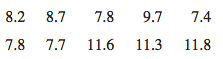
\includegraphics{../../fig/fbeams.png}
\end{center}
\item At $\alpha = 0.01$, I will test the hypothesis that the true mean flexural strength is 10 MPa.
\end{itemize}
\end{frame}

\begin{frame}
\frametitle{Example: concrete beams} \small
\begin{enumerate}[1. ]
\item $H_0: \mu = 10 MPa$, $H_a: \mu \ne 10 MPa$, where $\mu$ is the true mean flexural strength of the beams. 
\pause \item $\alpha = 0.01$.
\pause \item Since this is a two-sided test, I will use a two-sided confidence interval:
\pause \begin{align*}
\left (\ov{x} - t_{n - 1 , \ 1 - \alpha} \frac{s}{\sqrt{n}}, \ \ov{x} + t_{n - 1 , \ 1 - \alpha} \frac{s}{\sqrt{n}} \right )
\end{align*}
\pause I am assuming the data points $x_1, \ldots x_n$ were independently drawn from $N(\mu, \sigma^2)$.
\pause \item From before, we calculated the confidence interval to be (7.393, 11.007).
\pause \item Since 10 MPa is in the interval, we fail to reject $H_0$.
\pause \item There is not enough evidence to conclude that the true mean flexural strength is different from 10 MPa. 
\end{enumerate}
\end{frame}



\begin{frame}
\frametitle{Your turn: paint thickness}
\begin{itemize}
\item Consider the following sample of observations on coating thickness for low-viscosity paint: 
\pause \begin{tabular}{cccccccc}
0.83 & 0.88 & 0.88 & 1.04 & 1.09 & 1.12 & 1.29 & 1.31 \\
1.48 & 1.49 & 1.59 & 1.62 & 1.65 & 1.71 & 1.76 & 1.83
\end{tabular} \q
\pause \item Using $\alpha = 0.1$, test the hypothesis that the true mean paint thickness is 1.00 mm.
\pause \item Note: the 90\% confidence interval for the true mean paint thickness was calculated from before as  (1.201, 1.499).
\end{itemize}
\end{frame}


\begin{frame}<handout:\answers>
\frametitle{Answers: paint thickness} \small
\begin{enumerate}[1. ]
\item $H_0: \mu = 1.00$, $H_a: \mu \ne 1.00 mm$, where $\mu$ is the true mean paint thickness. 
\pause \item $\alpha = 0.1$.
\pause \item Since this is a two-sided test, I will use a two-sided confidence interval:
\pause \begin{align*}
\left (\ov{x} - t_{n - 1 , \ 1 - \alpha} \frac{s}{\sqrt{n}}, \ \ov{x} + t_{n - 1 , \ 1 - \alpha} \frac{s}{\sqrt{n}} \right)
\end{align*}
I am assuming the data points $x_1, \ldots x_n$ were independently drawn from $N(\mu, \sigma^2)$.
\pause \item From before, we calculated the confidence interval to be (1.201, 1.499).
\pause \item Since 1.00 mm is not in the interval, we reject $H_0$ and conclude $H_a$.
\pause \item There is enough evidence to conclude that the true mean paint thickness is not 1.00 mm.
\end{enumerate}
\end{frame}

\begin{frame}
\frametitle{Next time}
\begin{enumerate}[1. ]
\item Review of hypothesis testing with confidence intervals.
\pause \item Hypothesis testing with critical values. 
\pause \item Hypothesis testing with p-values.
\end{enumerate}
\end{frame}

\end{document}
